\section{$\sigma_{\mathrm{CX}}$ and $\sigma_{\mathrm{ABS}}$ extraction}\label{sec:xsec}
As was mentioned in Sec. \ref{section:calibration}, our simulation is based on the \textsc{Geant4} package which uses the Bertini cascade model for modeling pion inelastic interactions but also handles other complex aspects of the analysis such as the geometrical description of the detectors. In order to estimate the number of signal ($N_{\mathrm{CX}}^{\mathrm{MC}}$) and background ($N_{\mathrm{BG}}^{\mathrm{MC}}$) events predicted by the different models shown in Sec. \ref{sec:physics} without having to rewrite the simulation using each toolkit, a scheme was developed to replace the detector simulation with a set of 2D selection, rejection, and mis-reconstruction efficiencies in momentum and angle bins of the outgoing particles and presented in Sec. \ref{sec:efficiencies}. These were then applied to the predictions from \textsc{Neut} and \textsc{Fluka} obtained using thin target ($\sim$1 mm) simulations and a nominal model was selected in Sec \ref{sec:nominal}.

%After the event selection described above, 
The measured $\sigma_{\mathrm{CX}}$ was obtained for each model from $N_{\mathrm{CX}}^{\mathrm{MC}}$, $N_{\mathrm{BG}}^{\mathrm{MC}}$, and the corresponding predicted CX cross section $\sigma_{\mathrm{CX}}^{\mathrm{MC}}$ following Eq. (\ref{eqn:xsec_calc}). $\sigma_{\mathrm{ABS}}$ was obtained by subtracting $\sigma_{\mathrm{CX}}$ from $\sigma_{\mathrm{ABS+CX}}$ obtained in \cite{duet}.

 \begin{equation} \label{eqn:xsec_calc}
 \begin{aligned}
 \sigma_{\mathrm{CX}} &= 
 \sigma_{\mathrm{CX}}^{\mathrm{MC}}
 \times \frac{N_{\mathrm{Data}}-N_{\mathrm{BG}}^{\mathrm{MC}}}{N_{\mathrm{CX}}^{\mathrm{MC}}} \\
 &\times
 \frac{1-R_{\mathrm{TiO}_2}^{\mathrm{Data}}}{1-R_{\mathrm{TiO}_2}^{\mathrm{MC}}}
 \times \frac{1}{1-f_{\mu}},
 \end{aligned}
 \end{equation} 

Corrections for the fraction of muons in the beam ($f_{\mu}$) and the fraction of interactions on TiO$_2$ nuclei ($R_{\mathrm{TiO}_2}^{\mathrm{Data}}$ and $R_{\mathrm{TiO}_2}^{\mathrm{MC}}$) were also applied. 

\subsection{Selection, rejection and mis-reconstruction efficiencies}\label{sec:efficiencies}

\begin{enumerate}
\item{{\bf $\pi^0$ selection efficiency:} the probability of a true CX event passing the selection criteria as a function of the outgoing $\pi^0$ momentum and angle is defined as the ratio of the distributions before and after the selection is applied. This selection efficiency is shown in Fig. \ref{fig:pi0_selection} for the $p_{\pi}$ = 201.6 MeV$/c$ setting as an example.}

\begin{figure}[h]
 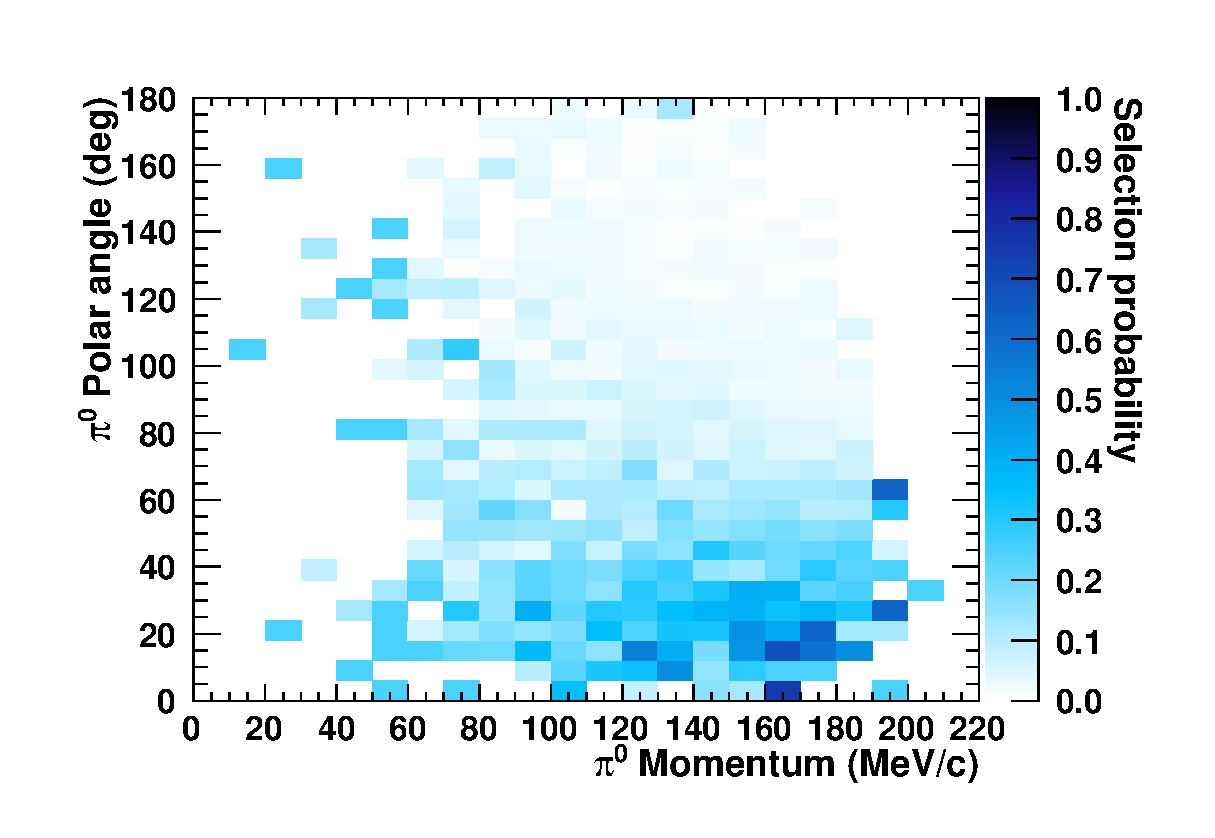
\includegraphics[width=86mm]{figures/Pi0SelectionEfficiency_200.eps}
 \caption{(Color online) Selection efficiency of true CX events as a function of the outgoing $\pi^{0}$ momentum and angle, for the $p_{\pi}$ = 201.6 MeV$/c$ setting.}
 \label{fig:pi0_selection}
\end{figure}

\item{{\bf Proton/neutron veto rejection:} the probability that an ejected proton or neutron will produce hits in the first two XY modules of CEMBALOS. Fig. \ref{fig:proton_rejection} shows the rejection efficiency for protons in the the 201.6 MeV$/c$ setting. The CEMBALOS forward acceptance ($<45^{\circ}$) can be clearly seen.}

\begin{figure}[h]
 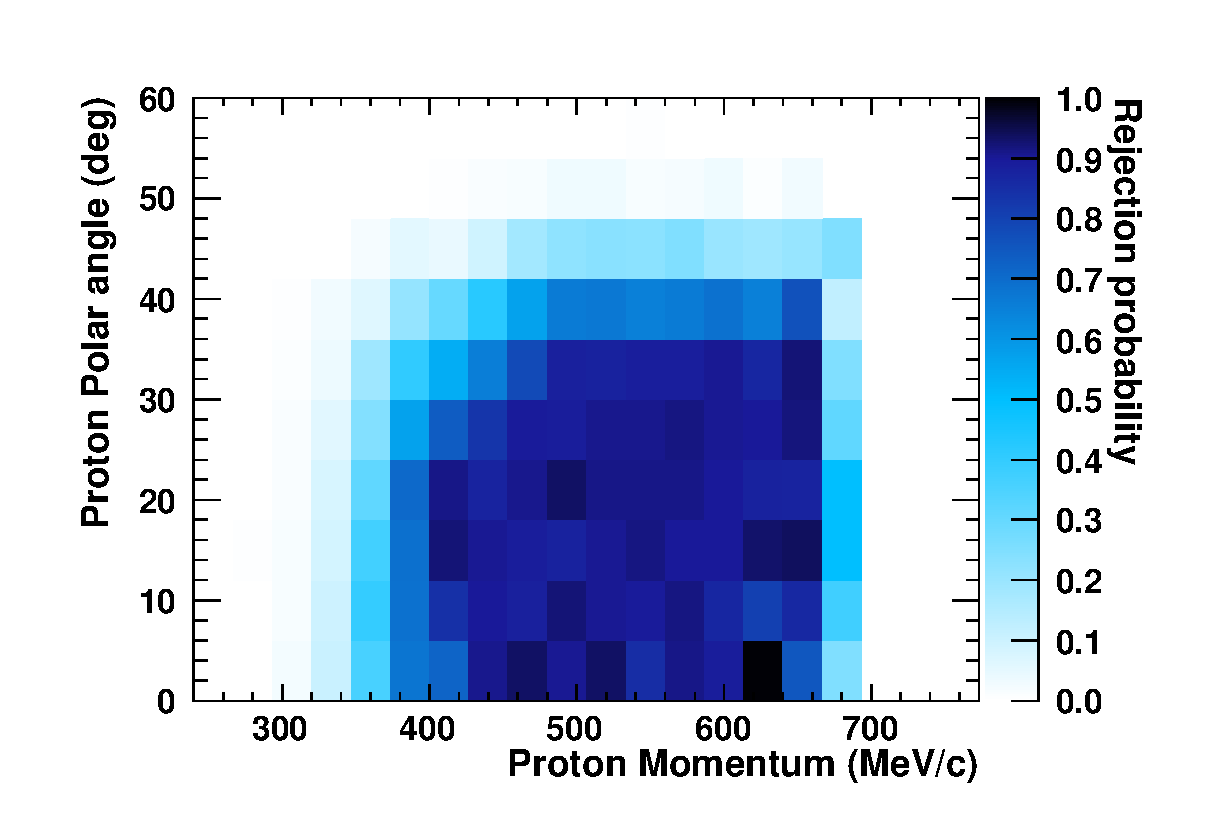
\includegraphics[width=86mm]{figures/ProtonRejectionEfficiency_200.eps}
 \caption{(Color online) Rejection probability of events where an ejected proton from ABS or quasi-elastic scattering fails the veto rejection criteria, as a function of its outgoing  momentum and angle, for the $p_{\pi}$ = 201.6 MeV$/c$ setting.}
 \label{fig:proton_rejection}
\end{figure}

\item{{\bf Proton mis-reconstruction:} the probability of a proton being mis-reconstructed as a ``pion-like'' track in PIA$\nu$O thus causing the event to be rejected.}

\item{{\bf $\pi^{+}$ mis-reconstruction and veto:} the probability of an outgoing $\pi^{+}$ following a quasi-elastic scatter to be mis-reconstructed in PIA$\nu$O as a ``proton-like'' track and then producing hits in the first two XY modules of CEMBALOS.}

\item{{\bf Neutron selection efficiency:} the probability of a neutron from an ABS event passing the selection criteria.}
\end{enumerate}

In this scheme a true CX event would be categorized as a signal event if: the $\pi^{0}$ is selected, the ejected proton(s) is not mis-reconstructed as a ``pion-like'' track in PIA$\nu$O, and the ejected nucleons do not trigger the veto rejection. On the other hand, an ABS or quasi-elastic scattering event would be categorized as a background event if: a neutron is selected, any outgoing $\pi^{+}$ is mis-reconstructed as a proton, all ejected proton(s) are not mis-reconstructed in PIA$\nu$O as ``pion-like'', and the the ejected nucleons do not trigger the CEMBALOS veto rejection. 

\subsection{Selection of nominal model}\label{sec:nominal}

The results of applying this scheme to model predictions from various models are summarized in Table \ref{tbl:eff_scheme_results} for each momentum setting. In addition to \textsc{Neut} and \textsc{Fluka}, the scheme was applied to the \textsc{Geant4} model prediction calculated from a thin target simulation (independent of the DUET simulation) as a means of validation of the procedure. The predictions of $N_{\mathrm{CX}}^{\mathrm{MC}}$ for \textsc{Geant4} agree with $N_{\mathrm{CX}}^{\mathrm{G4}}$ from Table \ref{tbl:short_event_summary} within $\sim$3\%, while $N_{\mathrm{BG}}^{\mathrm{MC}}$ were underestimated as not all sources of background were included in the scheme. These are discussed in Sec. \ref{sec:background}.
\begin{table}[htbp]
\begin{center}
\begin{tabular}{c|c|c|c|c|c}
%\noalign{\hrule height 1pt}                                                                                                                       
\hline
$p_{\pi}$ [MeV$/c$] & Model & $\sigma_{CX}^{MC}$ [mb] &  $N_{\mathrm{CX}}^{\mathrm{MC}}$  &  $N_{\mathrm{BG}}^{\mathrm{MC}}$  &  $\sigma_{CX}$ [mb] \\ \hline
\multirow{4}{*}{201.6} %& DUET & 34.3 & 60.4 & 8.7 & 59.1 \\
& \textsc{Geant4} & 36.7 & 63.3 & 6.1 & 58.0 \\
& \textsc{Fluka} & 55.5 & 122.2 & 6.3 & 45.3 \\
& \textsc{Neut} & 50.5 & 83.0 & 4.5 & 61.8 \\ \hline

\multirow{4}{*}{216.6} %& DUET & 34.9 & 15.8 & 2.4 & 42.5 \\
& \textsc{Geant4} & 37.5 & 16.5 & 2.0 & 41.6 \\
& \textsc{Fluka} & 59.5 & 32.5 & 1.5 & 34.4  \\
& \textsc{Neut} & 55.7 & 24.2 & 1.5 & 43.5 \\ \hline

\multirow{4}{*}{237.2} %& DUET & 36.8 & 75.9 & 11.1 & 68.2 \\
& \textsc{Geant4} & 39.6 & 80.0 & 9.7 & 65.4 \\
& \textsc{Fluka} & 61.7 & 149.4 & 5.8 & 56.1 \\
& \textsc{Neut} & 57.5 & 111.7 & 6.1 & 69.8 \\ \hline

\multirow{4}{*}{265.5} %& DUET & 41.3 & 87.1 & 10.5 & 72.4 \\
& \textsc{Geant4} & 44.7 & 88.8 & 9.6 & 71.4 \\
& \textsc{Fluka} & 62.4 & 143.5 & 5.0 & 63.7 \\
& \textsc{Neut} & 57.9 & 129.4 & 6.9 & 64.8 \\ \hline

\multirow{4}{*}{295.1} %& DUET & 41.6 & 119.4 & 12.8 & 56.5 \\
& \textsc{Geant4} & 45.1 & 122.5 & 12.7 & 55.1 \\
& \textsc{Fluka} & 58.5 & 176.2 & 5.6 & 52.0 \\
& \textsc{Neut} & 58.3 & 170.3 & 8.4 & 52.7 \\ \hline
%\noalign{\hrule height 1pt}
\end{tabular}
\caption{Predicted $N_{\mathrm{CX}}^{\mathrm{MC}}$, $N_{\mathrm{BG}}^{\mathrm{MC}}$ and extracted CX cross section $\sigma_{\mathrm{CX}}$ obtained from applying the efficiency scheme to \textsc{Geant4}, \textsc{Fluka}, and \textsc{Neut} model predictions. See text for discussion.}
\label{tbl:eff_scheme_results}
\end{center}
\end{table}

The differences in the extracted cross section among models range from 21.9\% at $p_{\pi}$ = 201.6 MeV$/c$ to 5.7\% at $p_{\pi}$ = 295.1 MeV$/c$, with \textsc{Fluka} and \textsc{Geant4} being the extreme case scenarios. This is consistent with the model comparison from Fig. \ref{fig:pi0kinem}. Considering the good agreement between \textsc{Fluka} and the external data in Fig. \ref{fig:pi0kinem}, the results from applying the efficiency scheme to \textsc{Fluka}, with the $N_{\mathrm{BG}}^{\mathrm{MC}}$ prediction scaled up to increase the additional backgrounds not included in the scheme, were chosen as our nominal result.